\scanpage{28}
\mspage{26}
Ceci montre que décidément, il faut en rabattre, et que dans le titre du Chapitre et les considérations de 2.2., c'est à condition de prendre partout des isocristaux qu'il reste une chance d'une théorie du genre de celle envisagée précédemment. Il est fort possible d'ailleurs que la notion de isocristal que j'ai adoptée est encore trop restrictive, en ce sens que dans la description de 1.13. il faudra peut-être prendre des stratifications en caractéristique nulle qui ne se prolongeraient pas nécessairement sur le schéma formel sur $W$ = vecteurs de Witt tout entier. C'est une analyse soigneuse du calcul-clef de Washnitzer-Monsky qui devrait permettre de tirer cette question au clair.
\margin{\figure{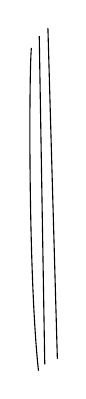
\begin{tikzpicture}
\draw (0,0) .. controls (-0.13,1.2) and (-0.12,3.8) .. (-0.09,4.1);
\draw (0.08,0.08) -- (0.01,4.25);
\draw (0.24,0.15) -- (0.12,4.35);
\end{tikzpicture}}}

2.8. Il se pose la question, d'autre part, pour quels schémas abéliens les énoncés 1º et 3º de 2.4, 2.5. et 2.6. sont valables, en dehors du cas déjà signalé: $S$ de caractéristique nulle.
\figure{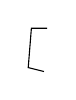
\begin{tikzpicture}\draw (0.2,0.55) -- (0,0.55) -- (-0.04,0.05) -- (0.16,0);\end{tikzpicture}}
\deleted{J'aurais assez tendance à croire que si $A$ est une VA définie sur un corps $k$ de car.$p>0$, alors ce qu'on veut (savoir l'indépendance de $G(B)$ d'un relèvement infinitésimal choisi $B$ de $A$) est vrai, pour tout anneau artinien de corps résiduel $k$, \uline{si et seulement si} $A$ est ``ordinaire'' i.e. a sur la clôture algébrique de $k$ le nombre maximum de points d'ordre $p$. Notes qu'il n'est pas nécessaire de supposer $k$ parfait (la question est manifestement géométrique), donc le groupe \deleted{formel} \inserted{p-divisible} de $A$ sur $k$ ne se décompose pas nécessairement en produit d'un étale par un infinitésimal. On aurait alors, pour de telles VA au moins, la description très explicite des relèvements infinitésimaux en termes du relèvement d'une filtration d'un module à la Dieudonné. Cette conjecture semble raisonnable car on a fait ce qu'il fallait pour éliminer des ennuis comme dans l'exemple de 2.7., d'autre part cela s'harmonise fort bien avec le tapis Serre des relèvements canoniques \inserted{et des modules} de variétés abéliennes du type ``ordinaire''.

Il serait évidemment tentant d'espérer qu'un énoncé du même type serait vrai pour une base quelconque, pourvu que toutes les fibres de $A/S$ soient des VA ordinaires. Mais cela est certainement faux avec cette généralité, même pour des schémas elliptiques, essentiellement toujours pour les même rai-\inserted{sons.}}
\margin{Faux, \unsure{ce} n'est \uline{jamais} vrai en car $p>0$ !}
\margin{\figure{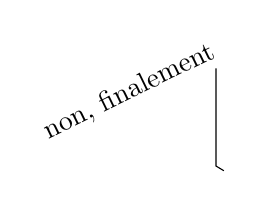
\begin{tikzpicture}
\draw (2.25,0) -- (2.15,0.06) -- (2.15,1.3);
\node[rotate=26] at (1.05,1.0) {non, \unsure{finalement}};
\end{tikzpicture}}}
\margin{27}
